% !Mode:: "TeX:UTF-8"

\documentclass[11pt, a4paper]{article}
%\usepackage{xltxtra,fontspec,xunicode}
\usepackage{amsmath}
\usepackage{amssymb}
\usepackage{breqn}
\usepackage{autobreak}
\usepackage{braket,mleftright}
\usepackage{amsfonts}
\usepackage[section]{placeins}
\usepackage{float}
\usepackage{siunitx}
\usepackage{graphicx}
\usepackage{subcaption}
\usepackage{mwe}
\usepackage{indentfirst}
\usepackage{caption}
\usepackage{physics}
\usepackage{geometry}
\usepackage{graphicx}
\usepackage{algorithm}% http://ctan.org/pkg/algorithm
\usepackage{algpseudocode}% http://ctan.org/pkg/algorithmicx

\geometry{top=1in, bottom=1in, left=1in, right=1in}
%\linespread{1.5}

\DeclareMathOperator*{\argmax}{argmax}
\DeclareMathOperator*{\argmin}{argmin}

\newcommand{\degc}{$\,^\circ$C}

\begin{document}

\title{Work Report}
\author{Zhuoran Qiao}
\date{\today}

\maketitle

\section{Introduction}

\paragraph{1} Developed a genetic algorithm based approach to simulate kinetics of co-transcriptional folding.
\paragraph{2} Tested effect of folding rate variation on folding population dynamics and $p_{unbound}$.


\section{Progress}
\subsection{Framework}
Various algorithms or programs have been developed to predict RNA folding pathway ultilizing force-field based simulations and multiple coarse grained energy landscape sampling methods built on Markov state model. Those present methods have succeeded in revealing multiscale dynamic events during RNA folding, however are either designed for only predicting
annealing dynamics or limited to RNA segments with length up to hundred bases. To quantitatively predict folding dynamics coupled with transcription,
we developed a genetic algorithm and chemical Master equation based approach, which is capable of capturing kilobase level kinetics.
 Our method is built on two following assumptions:
\paragraph{1} All populated RNA secondary structures (SS) are linkage of locally optimal or sub-optimal structures at various folding sites;
\paragraph{2} Global structural rearrangement of a partial RNA segment is permitted only if it's folding to the optimal SS on that segment.
\\

Formally, we denote a domain $D_{A,\,B}$ as a segment between base $A$ and $B$ that all contacts on that segment are local. For simplicity, we denote \textbf{foldon}
as domains with optimal secondary structures: $D^{foldon}_{A,\,B} = \text{MFE(sequence[A,B])}$. Note that $'.'$ is a trival example of foldon.
Our assumption 1 can be rewritten as
\begin{equation}
  D_{A,\,B} = D^{foldon}_{A, i_1} \oplus D^{foldon}_{i_1, i_2} \oplus ... \oplus D^{foldon}_{i_n, B}
\end{equation}
Where $\oplus$ represents a link operation. Note that all structural information of $D_{A,\,B}$ is encoded by the sequential representation $[A,\, i_1,\, ...,\, i_n,\, B]$;
 as a foldon is also a linkage of smaller foldons, there could be multiple way to represent $D_{A,\,B}$. Here we introduce \textbf{Irreducible Foldon Representation} (IFR) to be the
 sequential representations for which linkage of every adjacent foldons is not another foldon: $\forall k,\, D^{foldon}_{i_k, i_{k+1}} \oplus D^{foldon}_{i_{k+1}, i_{k+2}} \neq D^{foldon}_{i_{k}, i_{k+2}}$.
 Then the sufficient and necessary condition for structural rearrangement is

\begin{center}
  $\langle D^{u}_{A,\,B} | \hat{\mathbf{T}} | D^{v}_{A,\,B} \rangle \neq 0$ if and only if $\exists\, i,\,j$ satisfies

  $i,\,j \in D^{u}_{A,\,B}$.IFR, $i,\,j \in D^{v}_{A,\,B}$.IFR;

  $D^{u}_{A,\,i} = D^{v}_{A,\,i},\, D^{u}_{j,\,B} = D^{v}_{j,\,B}$;

  $D^{u}_{i,\,j} = D^{foldon}_{i,\,j}$ or $D^{v}_{i,\,j} = D^{foldon}_{i,\,j}$.

  Then $\langle D^{u}_{A,\,B} | \hat{\mathbf{T}} | D^{v}_{A,\,B} \rangle = \langle D^{u}_{i,\,j} | \hat{\mathbf{T}} | D^{v}_{i,\,j} \rangle$.
\end{center}

\subsection{Folding pathway identification \& Rate calculation} \label{section:rate}

Given two domains between which rearrangement is allowed, the task is to compute forward and backward rate constant
linking each other. Multiple methods to rigorously calculate the maximum likelihood during RNA folding have been reported;
here we proposed a computationally feasible approach: the forward free energy barrier is estimated by sum up all free energy associated
with old stacks unzipping and new loop forming; then rate constant $k_{uv} = \langle D^{u}_{A,\,B} | \hat{\mathbf{T}} | D^{v}_{A,\,B} \rangle $ is calculated by Arrhenius approximation $k_{uv} = k_0 \exp[-\frac{1}{RT}(\Delta G^{Stack}_{u}+\Delta G^{Loop}_{v})]$. 'New' and 'old' helices are identified by comparing elementary domains (defined as domains that cannot be decomposed to smaller valid domains) between reactant and product domains; identical elementary domains are excluded.

\subsection{Algorithm procedure}

During every iterative elongation step, an active species pool of strands with unique SS and diffrent population is updated. New candidate strands $D^{Candidate}_{0,\, L+\Delta L}$ with
length $L+\Delta L$ are generated by a recombination
process: for every old strand $D^{Strand}_{0, \text{ L}}$, all indices in its IFR is identified as possible rearrangement site, then its child strands is generated by linking partial domains
$D^{Strand}_{0, \text{ Site}}$ with a foldon $D^{foldon}_{\text{Site}, L+\Delta L}$ that terminated at $L+\Delta L$.

We assume that elongation will not change the inital population distribution
of secondary structures: child strands with the exact parental SS on $[0, L]$ ($D^{child}_{0, L+\Delta L} = D^{strand}_{0, L} \oplus D^{foldon}_{L, L+\Delta L}$) will also inherit the population of their parents.

After structual generation the rate matrix among all candidate strands within the new active species pool is calculated (see part \ref{section:rate}). Then the population
distribution of strands after elongation is computed by propagate the chemical master equation.

For the sake of computational efficiency, we introduce a cutoff $N $ as the size limit of the active species pool. After each elongation step, we impose a selection sweep on all active
strands; species with top $N $ fitness is reserved. In the current edition, we simply used population as the fitness function. Population of remaining strands within
the active pool is renormalized after selection.

Pseudocodes of the whole simulation procedure are as follows (Algorithm \ref{algorithm:1}):

\begin{algorithm}
  \begin{algorithmic}[1]
    \State Initalize ActivePool
    \While{$\text{sequence length} > \text{current length }$}
      \State $\text{OldPool} \gets \text{ActivePool }$
      \State $\text{renew ActivePool }$
      \State $\text{Current length} \gets \text{Current length} + dL$
      \State $\text{dt} \gets dL / k_T$ \Comment{Transcription time}
      \For{$\text{left boundary} \in \text{\{0, dL, 2dL, ..., Current length - dL\}}$}\Comment{Get all new foldons}
        \State $D^{foldon}_{\text{left boundary}, \text{ Current length}} \gets \text{numpy.mfe(sequence[left boundary, Current length]})$
      \EndFor
      \For{$\text{Strand} \in \text{OldPool }$}\Comment{Recombination}
        \For{$\text{Site} \in \text{Strand.IFR }$}
          \State $D^{Candidate}_{0,\text{Current length}} \gets D^{Strand}_{0, \text{ Site}} \oplus D^{foldon}_{\text{Site}, \text{ Current length}}$
          \If {$D^{Candidate}_{0,\text{Current length}} \in \text{ActivePool }$}
            \State $\text{update $D^{Candidate}_{0,\text{Current length}}$.IFR}$
          \Else
            \State $\text{add $D^{Candidate}_{0,\text{Current length}}$ to ActivePool}$
          \EndIf
          \If {$\text{site} = \text{Current length} - dL$}
            \State $\langle \text{ActivePool}.\textbf{population}\,|D^{Candidate}_{0,\text{Current length}}\rangle \gets \langle \text{OldPool}.\textbf{population}\,|D^{Strand}_{0, \text{ Site}}\rangle$
          \EndIf
        \EndFor
      \EndFor
      \For{$D^{\text{u}}_{0,\text{Current length}} \neq D^{\text{v}}_{0,\text{Current length}} \in \text{ActivePool}$}\Comment{Calculate new rate matrix}
        \State $\text{calculate  } D^{u}_{\text{rearrange}} ,\ D^{v}_{\text{rearrange}}$\Comment{Find all helices involved in rearrangement}
        \State $\langle D^{u}_{\text{rearrange}} | \hat{\mathbf{T}} |D^{v}_{\text{rearrange}} \rangle \gets k_0 \exp(-\frac{1}{RT}(\Delta G^{Stack}_{u}+\Delta G^{Loop}_{v}) )$
      \EndFor
      \State $\langle \text{ActivePool}.\textbf{population}\,|\, \gets \langle \text{ActivePool}.\textbf{population}\,|\, \exp(t\times\hat{\mathbf{T}}) $\Comment{Master equation}
      \State $\text{reserve top $N$ populated strands in ActivePool}$\Comment{Selection}
      \State $\text{renormalize }\langle \text{ActivePool}.\textbf{population}\,|$
    \EndWhile
  \end{algorithmic}
\caption{Co-transcriptional folding elongation procedure}\label{algorithm:1}
\end{algorithm}

\subsection{Results}

The only remaining free parameter to be determined is $k_0/k_T$, the ratio of pre-exponential factor in Arrhenius rate formulation and trancription rate ($nt\cdot s^{-1}$). I tuned $k_0/k_T$ from $10^{1}$ to $10^{15}$ and obtained the data for $k_0/k_T=\infty$ by calculate stationary distribution ($\frac{1}{Q}\exp(-G_i)$) after every elongation step for strand i in active pool.
 
\paragraph{Population analysis} For folA-WT four predominant local folding motifs within SD sequence are identified. Figure \ref{fig:local_foldings} shows exemplary secondary structures containing these motifs; figure \ref{fig:populations} shows evolution of these structure motifs during co-transcriptional folding with different $k_0/k_T$. Identical motifs are marked by the same color as in figure \ref{fig:local_foldings}. Surprisingly we noticed that when $k_0/k_T=\infty$, exchange between dominant motifs is very frequent at early stage of transcription, indicating the sensitivity of local structures on long-range contacts, and dependence of motif predominance on the limited timescale for folding.

\begin{figure*}
    \centering
    \begin{subfigure}[b]{0.475\textwidth}
   		\centering
    	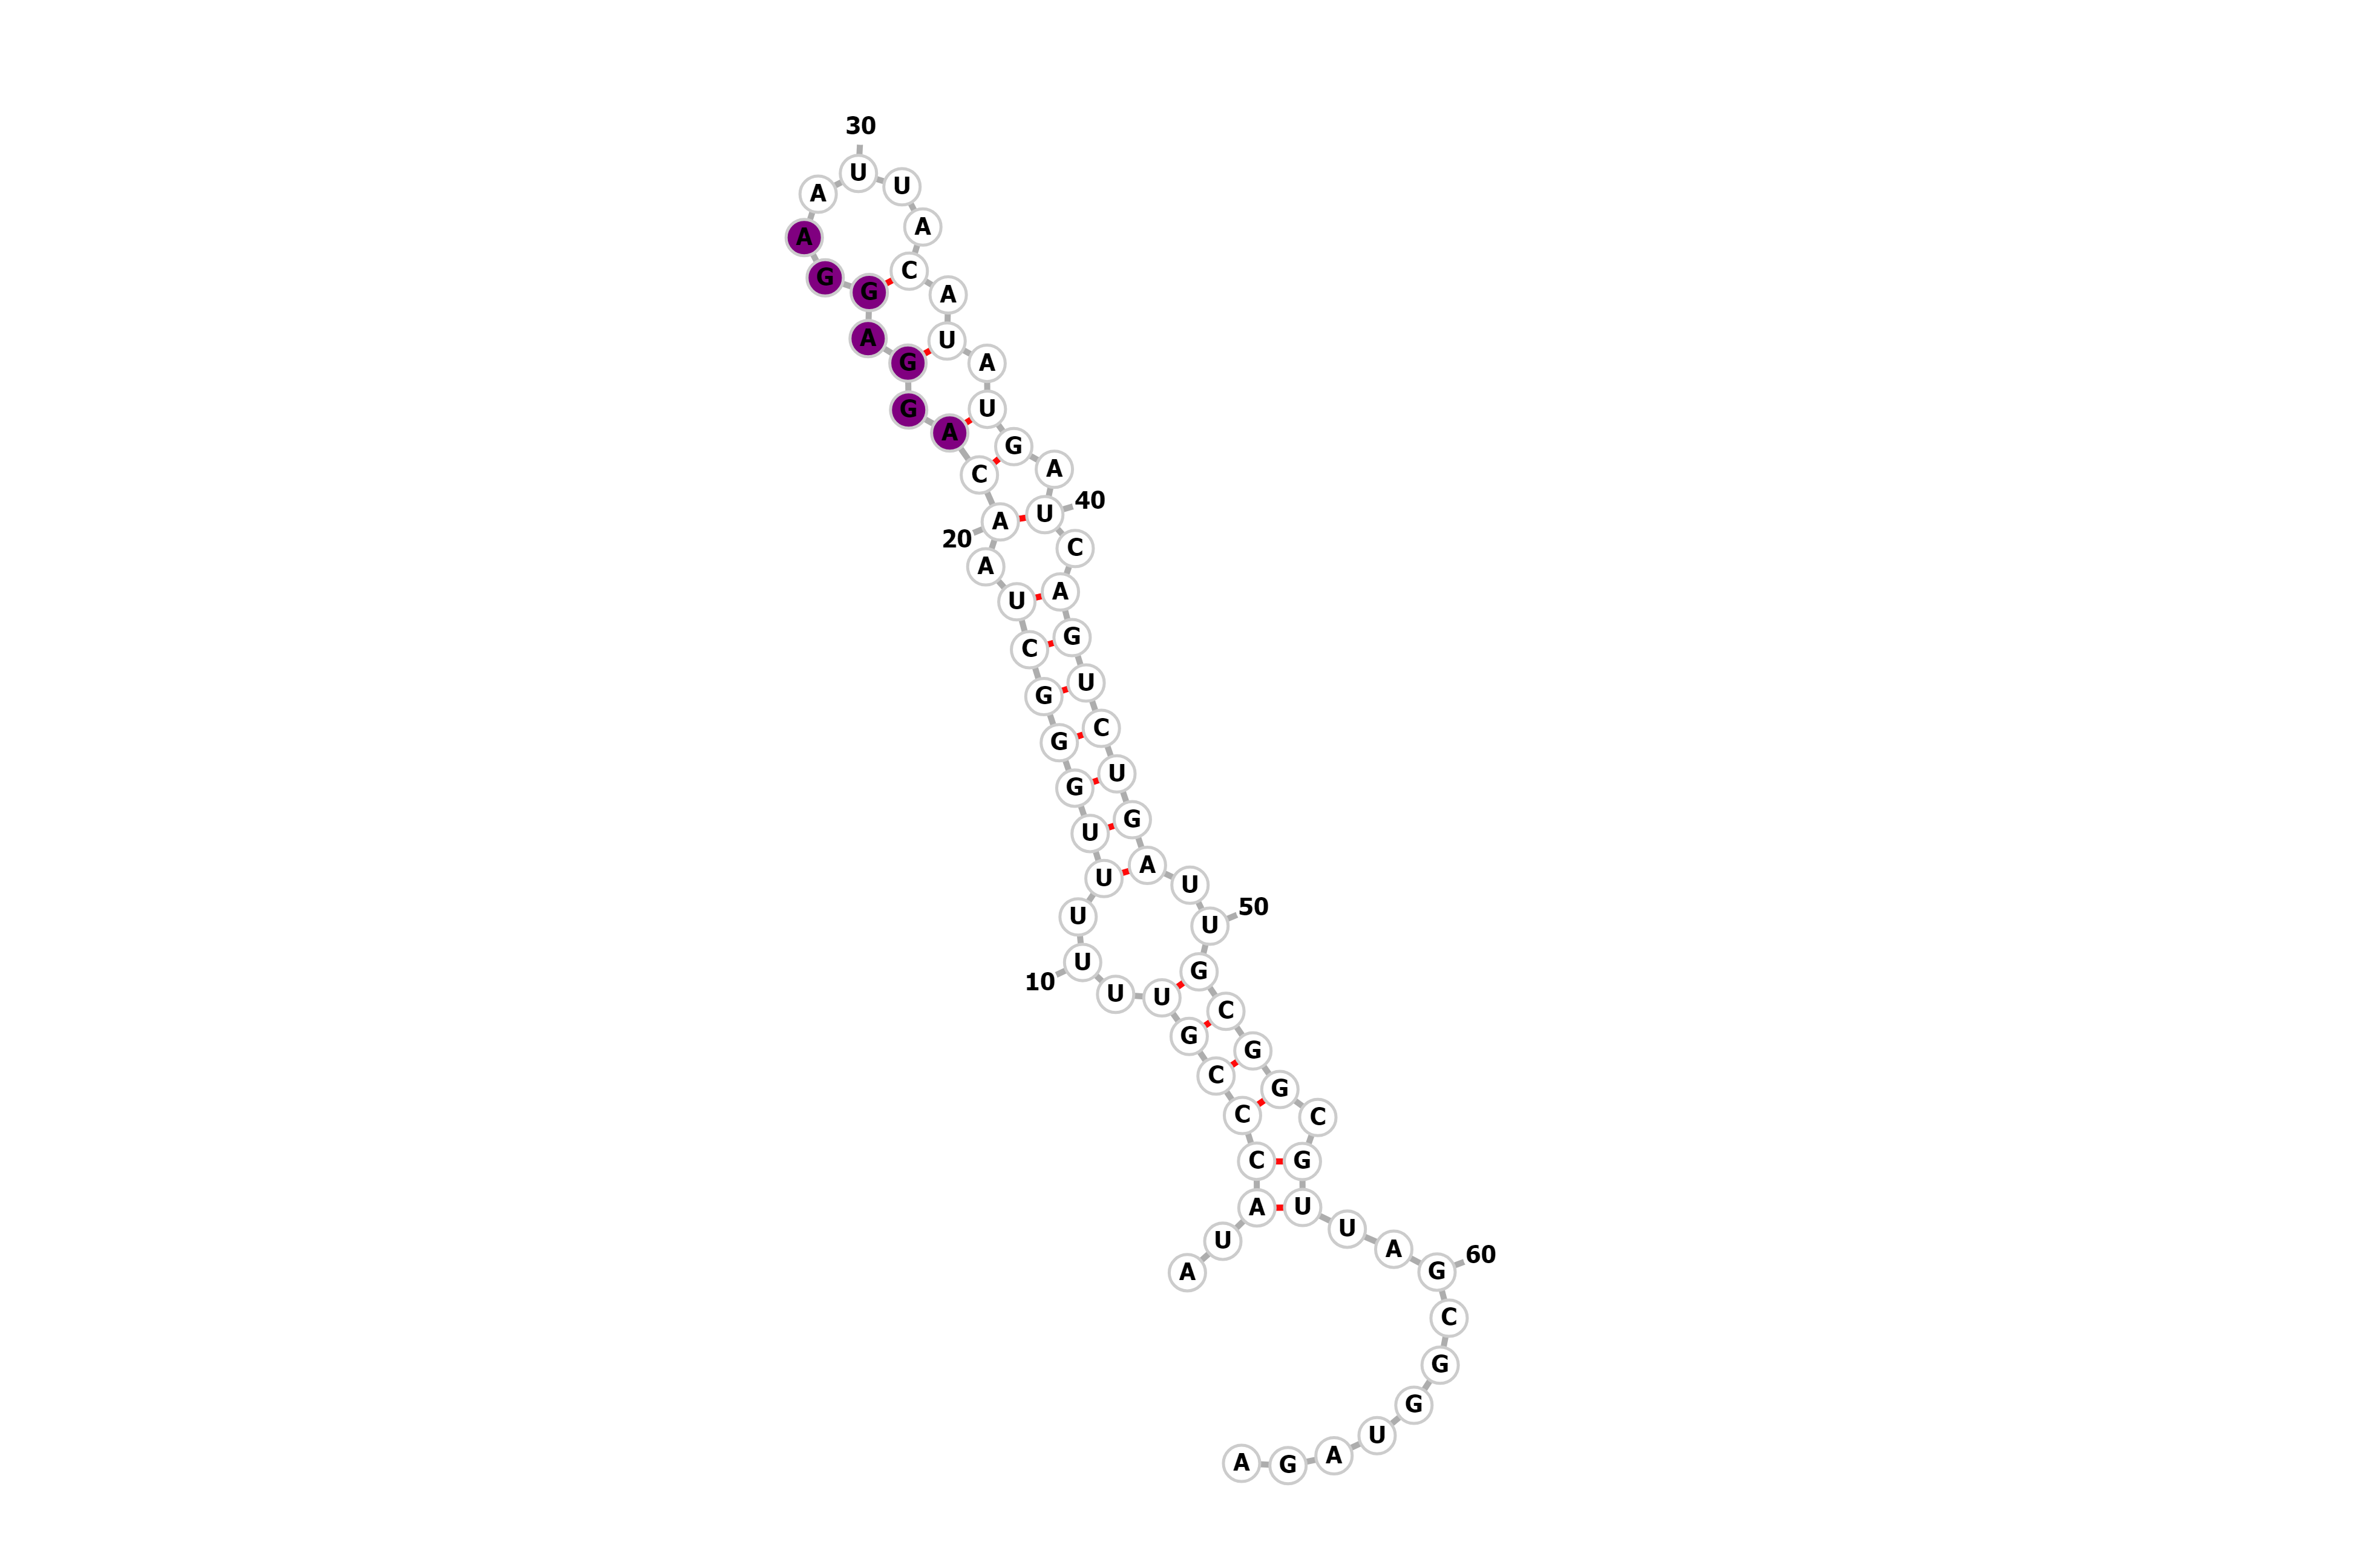
\includegraphics[width=\textwidth]{folding_example_purple}
    	\caption[]%
   		{{\small Motif 1}}    
    	\label{fig:mean and std of net14}
    \end{subfigure}
   	\hfill
    \begin{subfigure}[b]{0.475\textwidth}  
   		\centering 
   		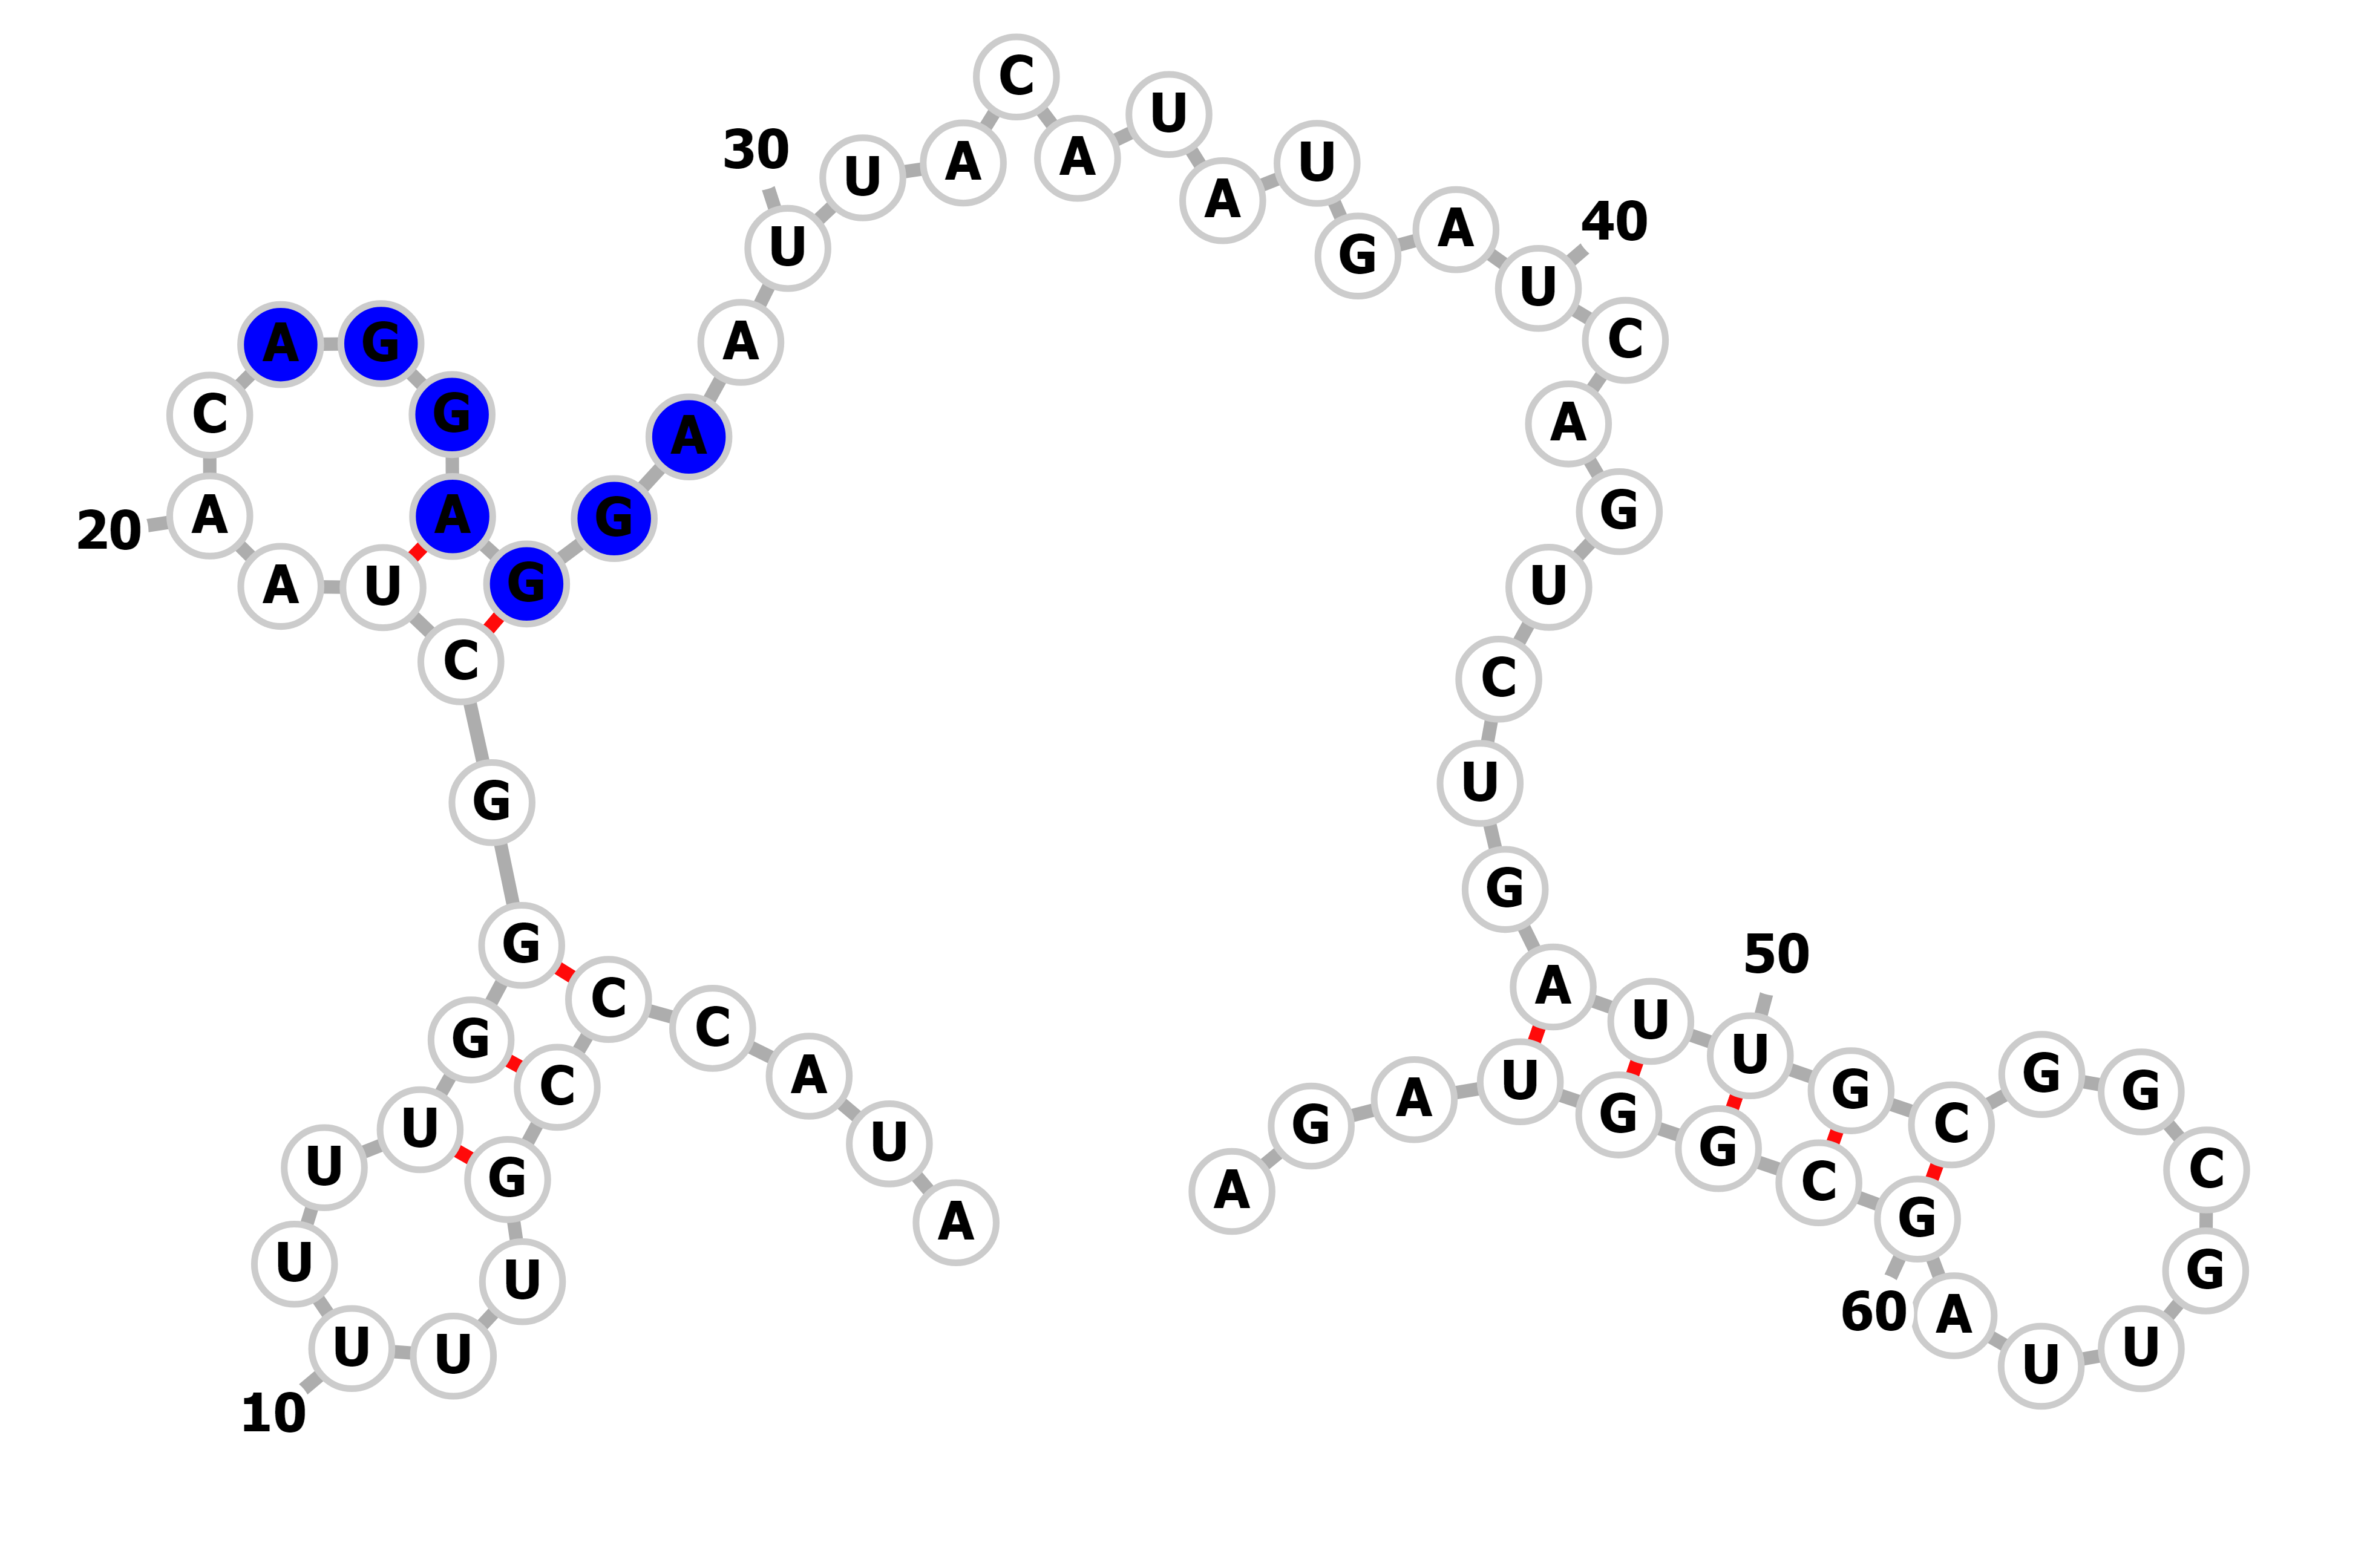
\includegraphics[width=\textwidth]{folding_example_blue}
    	\caption[]%
    	{{\small Motif 2}}    
   		\label{fig:mean and std of net24}
   	\end{subfigure}
   	\vskip\baselineskip
   	\begin{subfigure}[b]{0.475\textwidth}   
    	\centering 
    	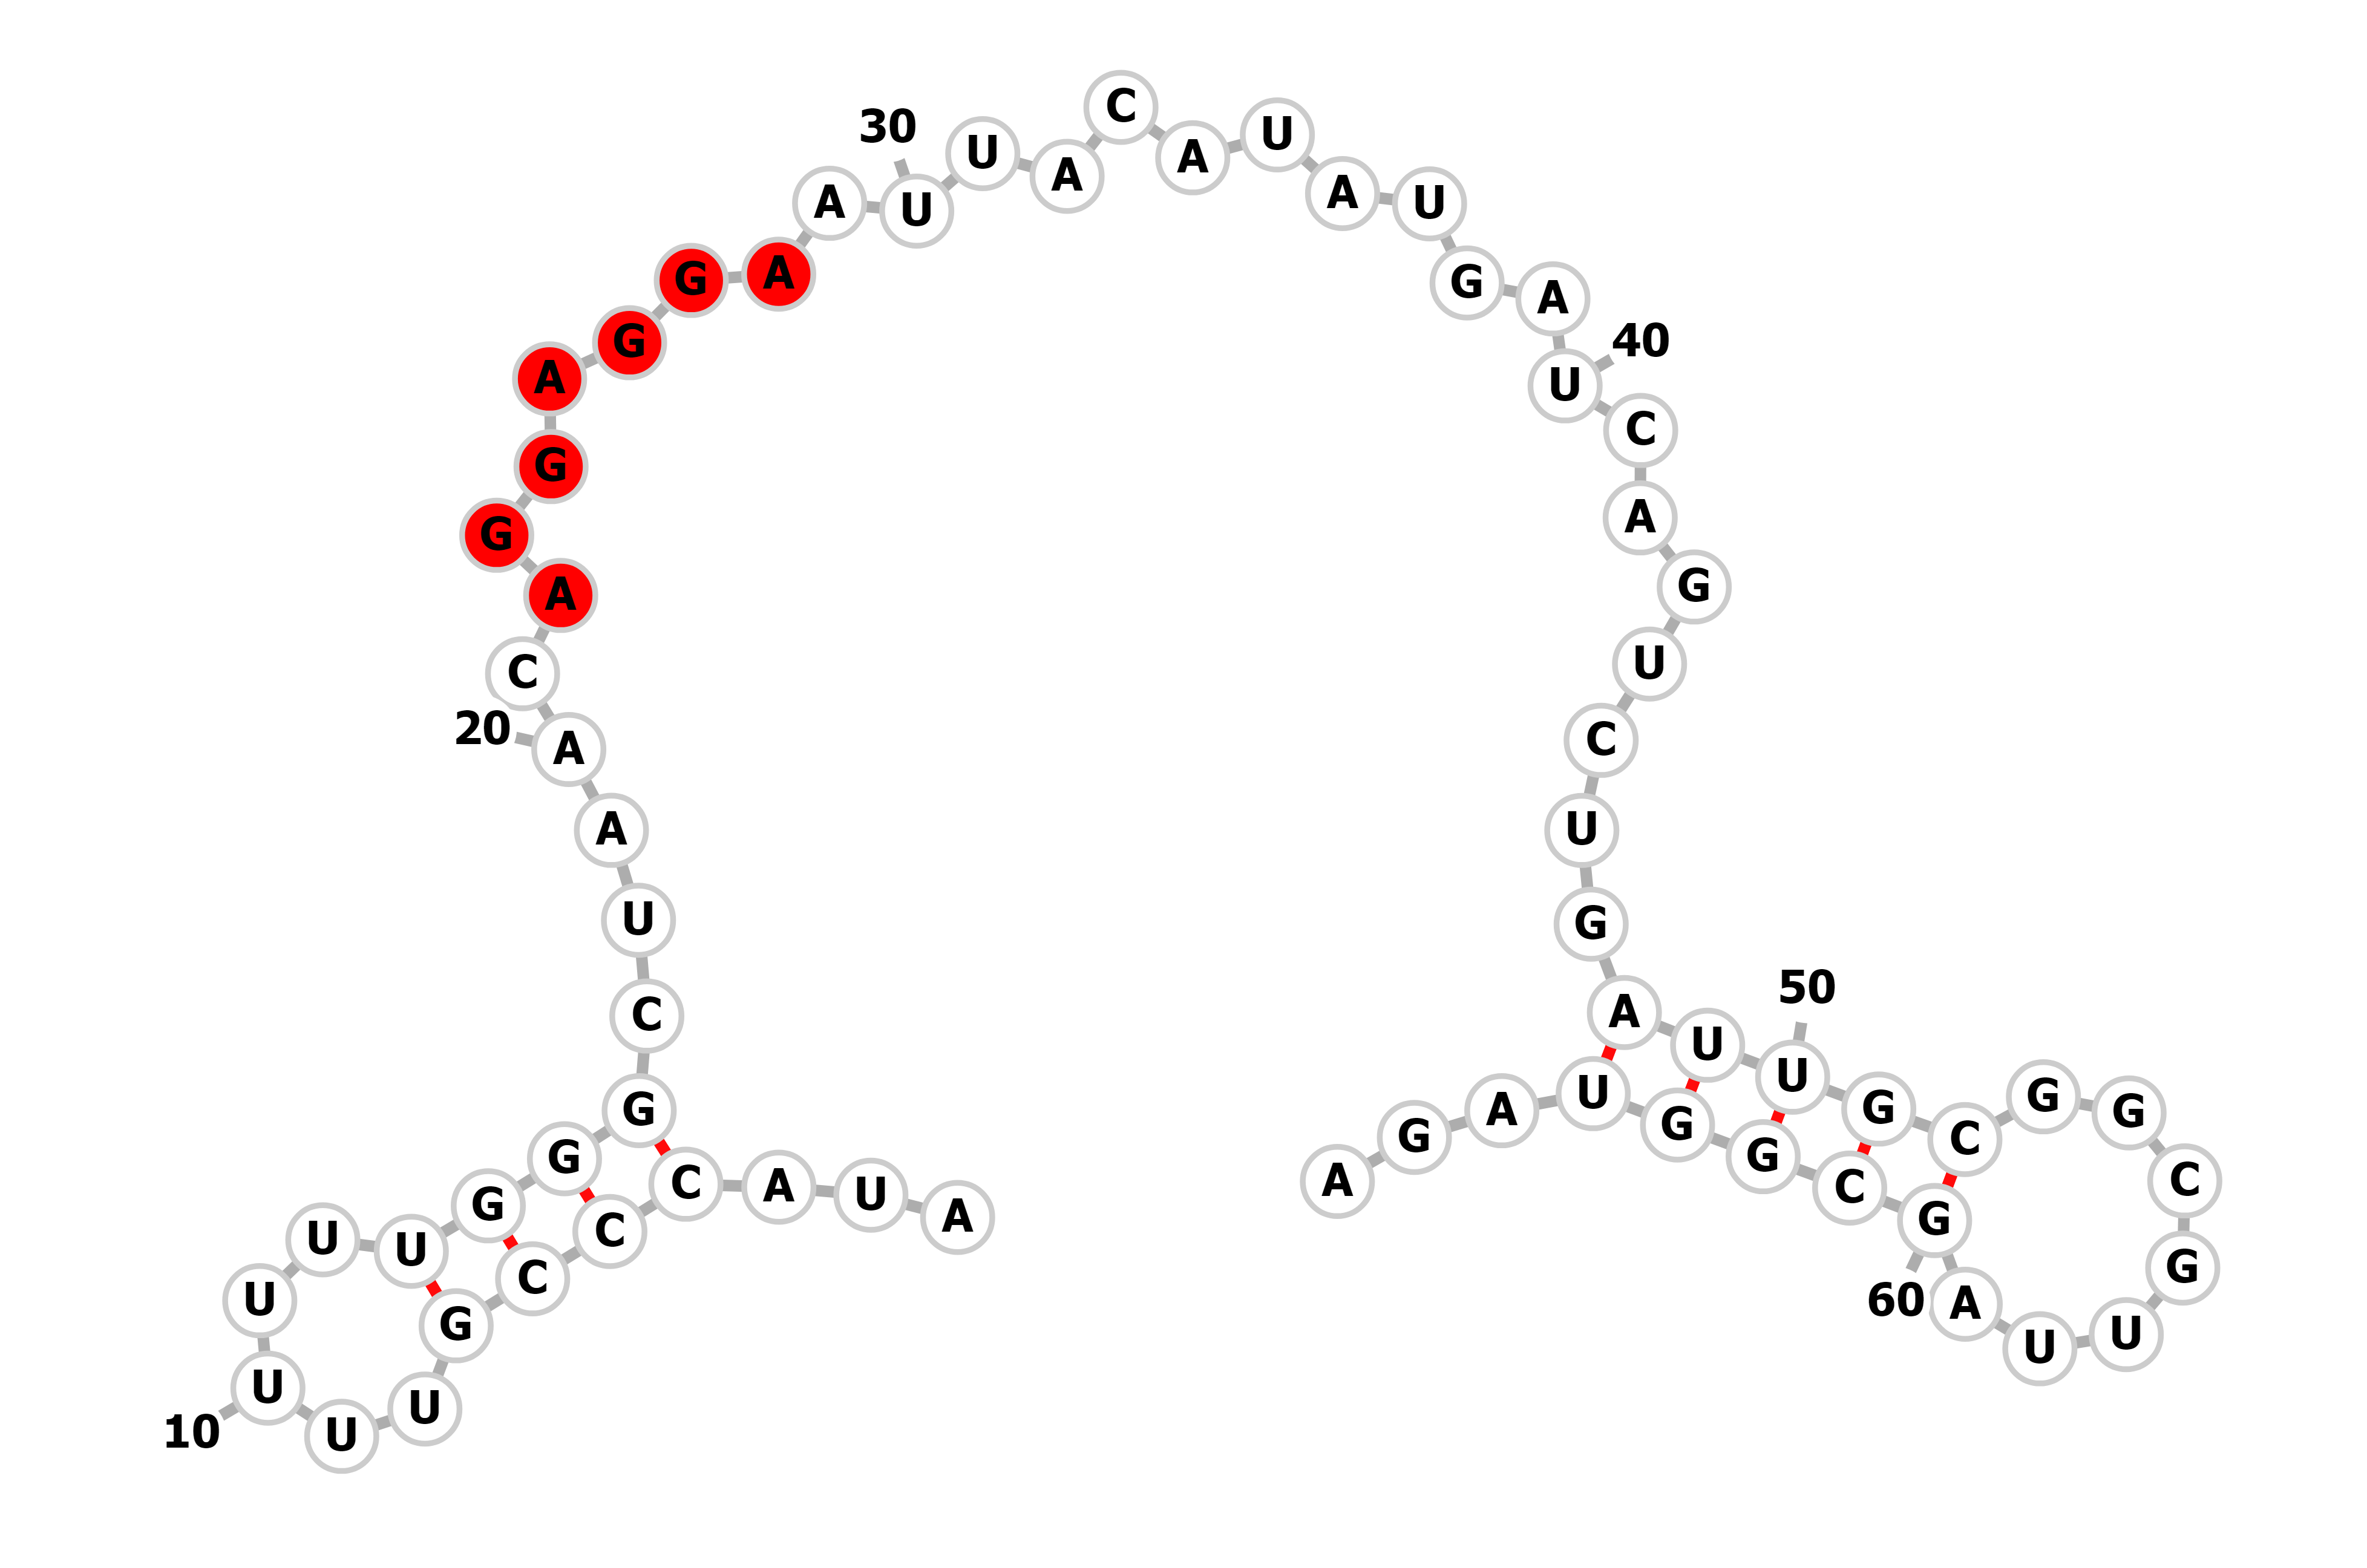
\includegraphics[width=\textwidth]{folding_example_red}
   		\caption[]%
   		{{\small Motif 3}}    
    	\label{fig:mean and std of net34}
    \end{subfigure}
   	\quad
   	\begin{subfigure}[b]{0.475\textwidth}   
   		\centering 
    	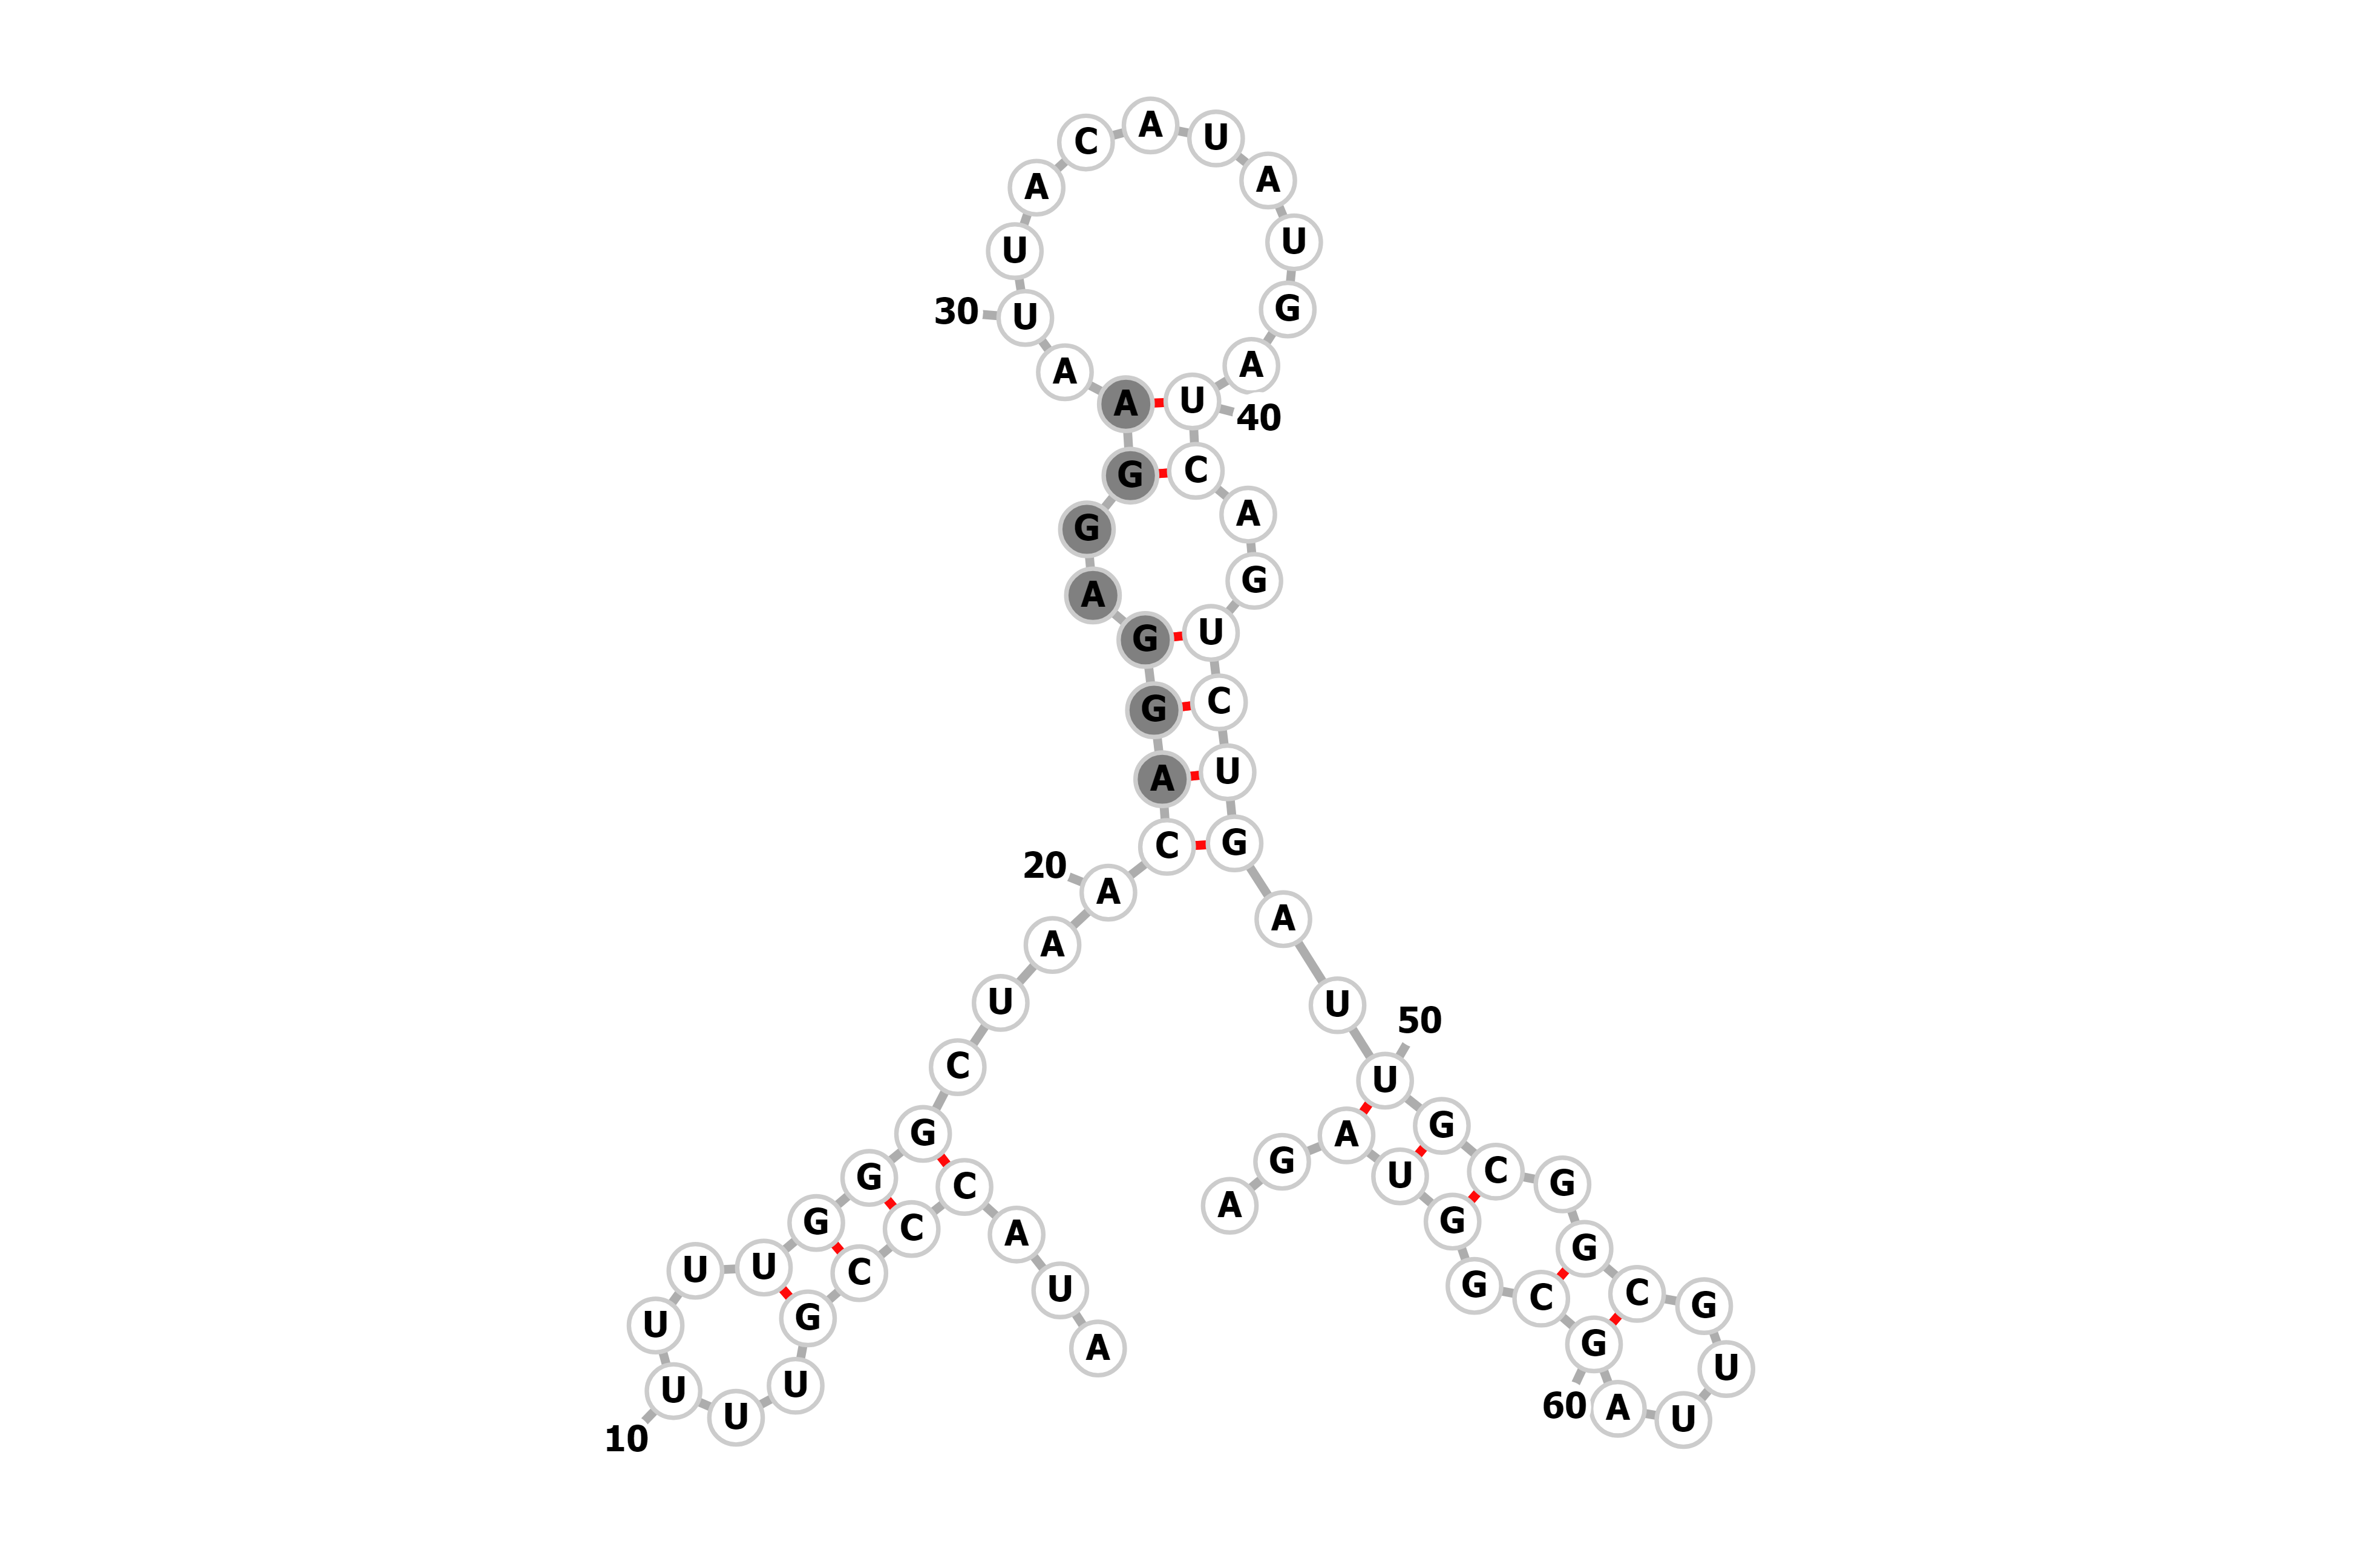
\includegraphics[width=\textwidth]{folding_example_grey}
    	\caption[]%
   		{{\small Motif 4}}    
   		\label{fig:mean and std of net44}
   	\end{subfigure}
    \caption[ Exemplary ss containing folding motifs within folA-WT Shine-Dalgarno sequence ]
   	{\small Exemplary ss containing folding motifs within folA-WT Shine-Dalgarno sequence} 
   	\label{fig:local_foldings}
\end{figure*}

\begin{figure*}[tph]
\centering
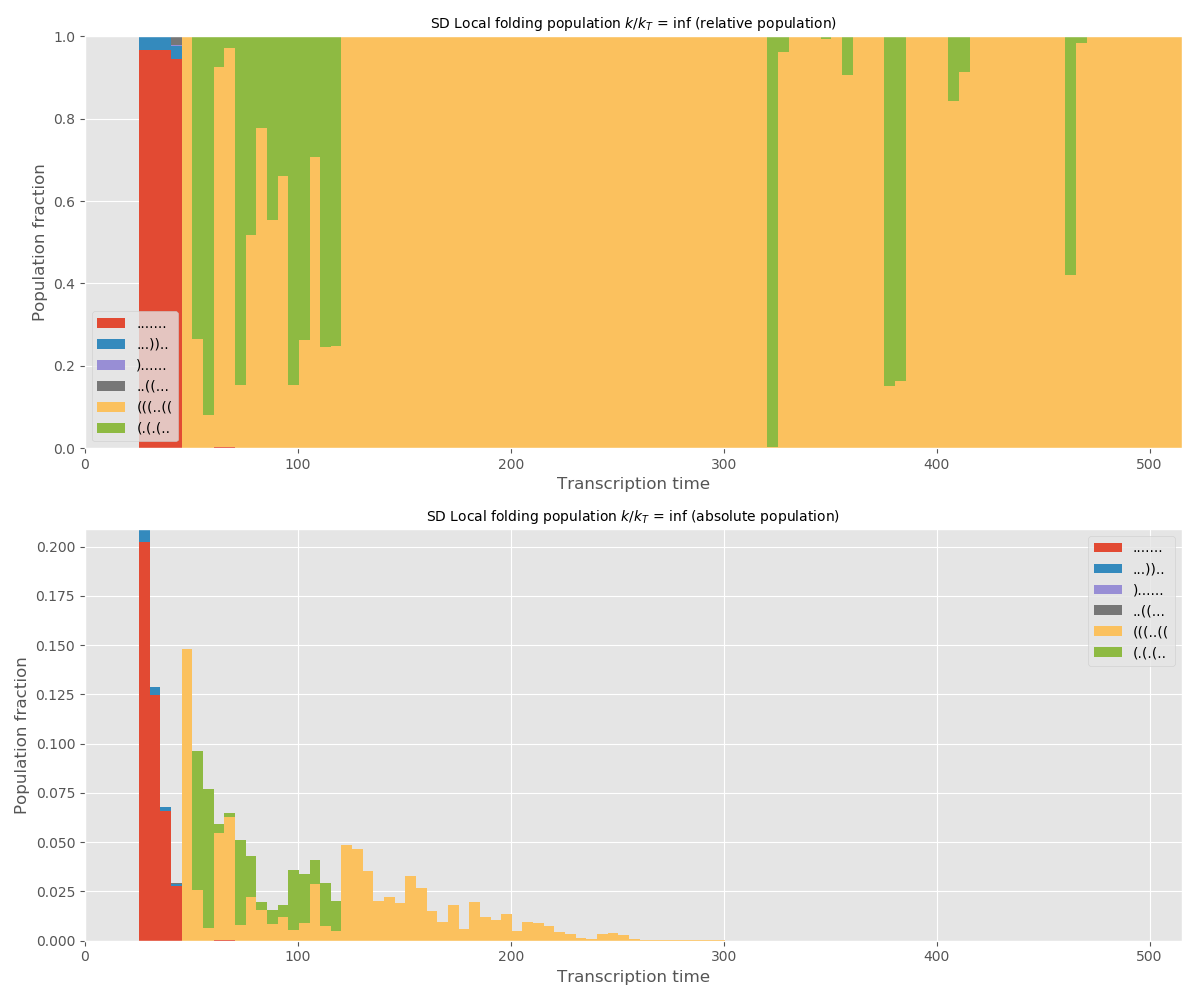
\includegraphics[width=\textwidth]{RNA_local_population_evolution_summary}
\caption[Population dynamics]{\small Population dynamics of four structrual motifs during co-transcriptional folding.}
\label{fig:populations}
\end{figure*}

\paragraph{$p_{unbound}$ analysis} We calculated $p_{unbound}$ with respect to transcription time and $k_0/k_T$ (Figure \ref{fig:RNA_p_unbound_SD_k_tuning}-\ref{fig:RNA_p_unbound_base[-14]_k_tuning}). Deviation of asymptotic behavior from equilibrium value (calculated by nupack.ppairs) is possiblly due to the limited set of foldons (only used mfe to obtain current results).

\begin{figure}
	\centering
	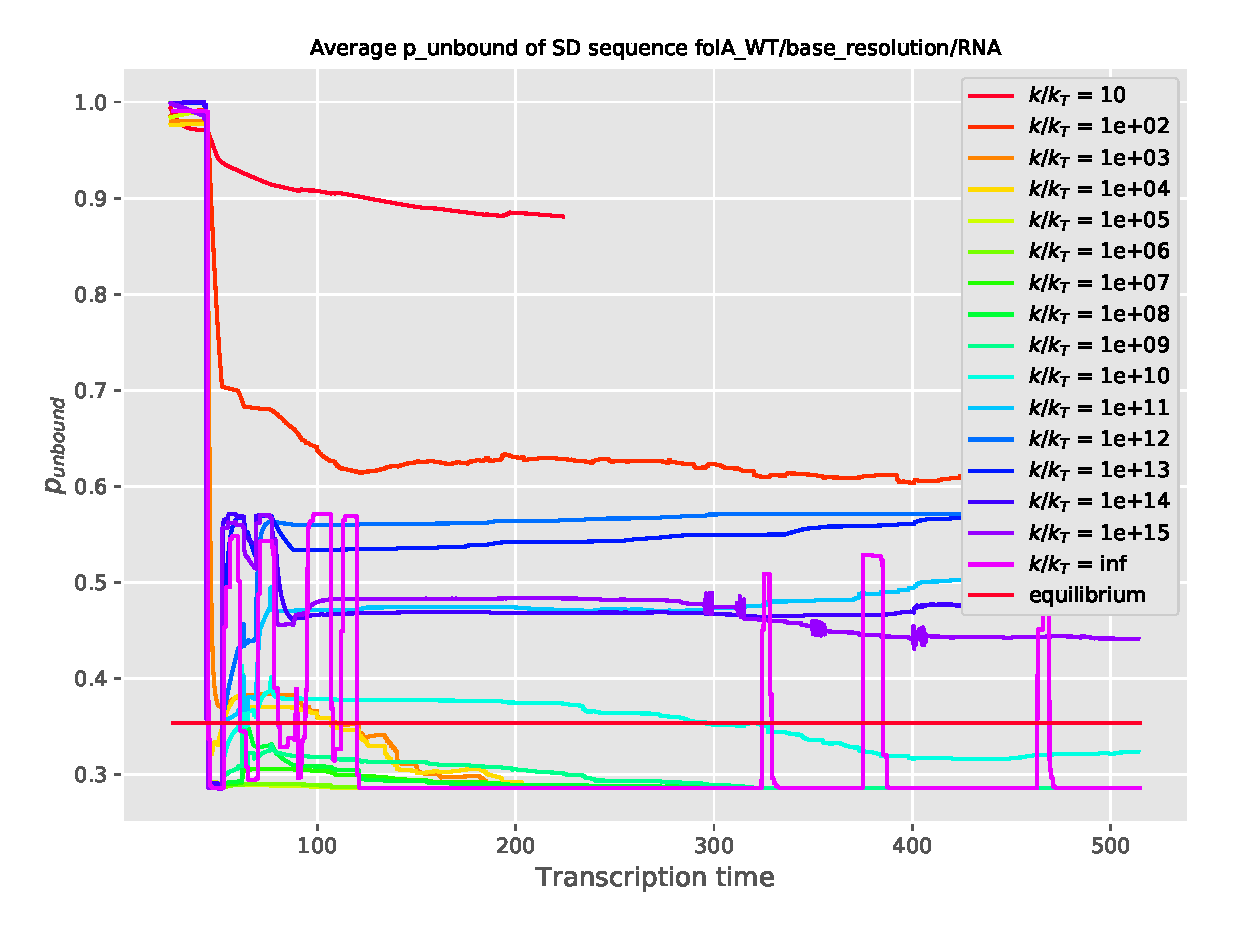
\includegraphics[width=\linewidth]{p_unbound/RNA_p_unbound_SD_k_tuning}
	\caption{}
	\label{fig:RNA_p_unbound_SD_k_tuning}
\end{figure}
\begin{figure}
\centering
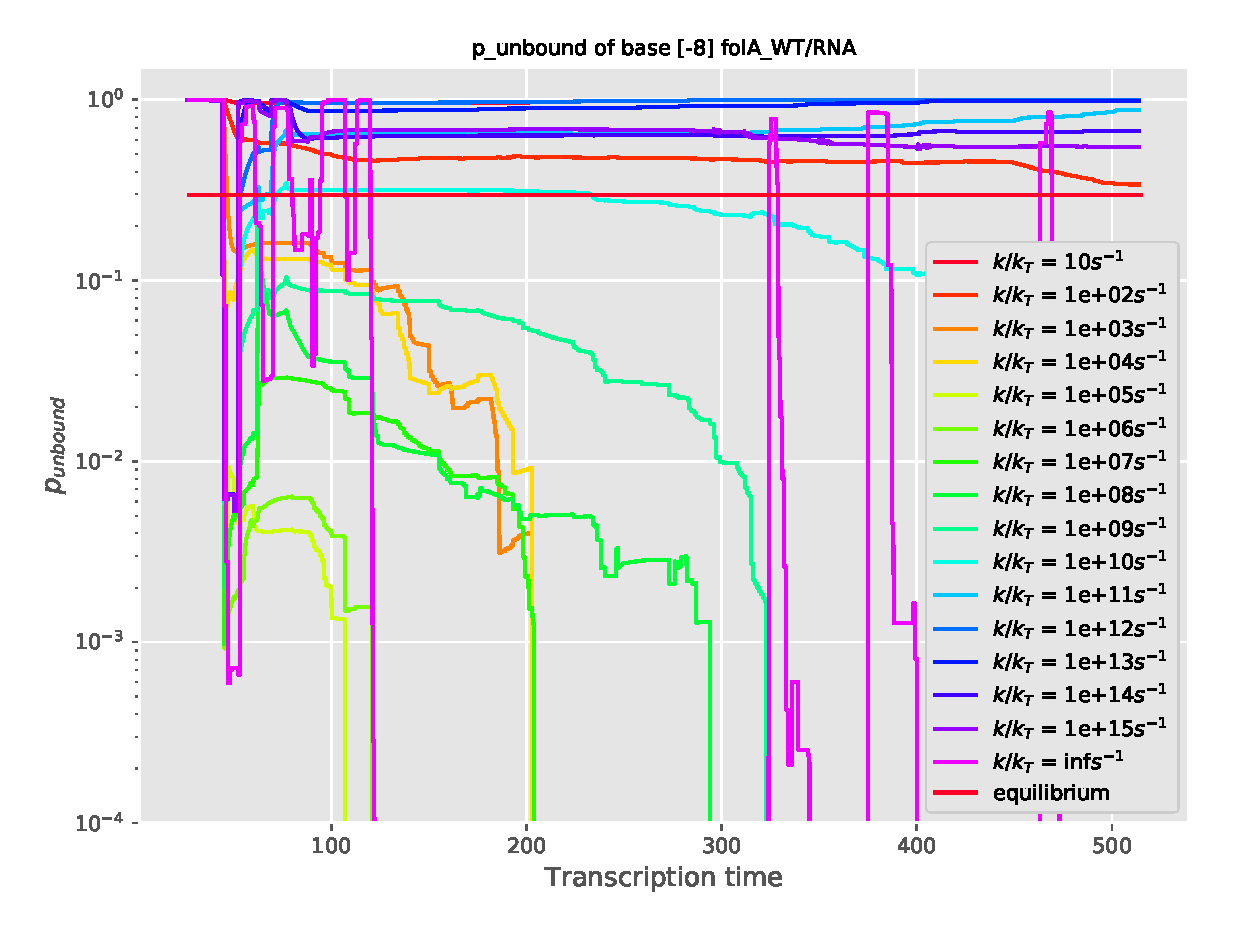
\includegraphics[width=\linewidth]{p_unbound/RNA_p_unbound_base[-8]_k_tuning}
\caption{}
\label{fig:RNA_p_unbound_base[-8]_k_tuning}
\end{figure}
\begin{figure}
\centering
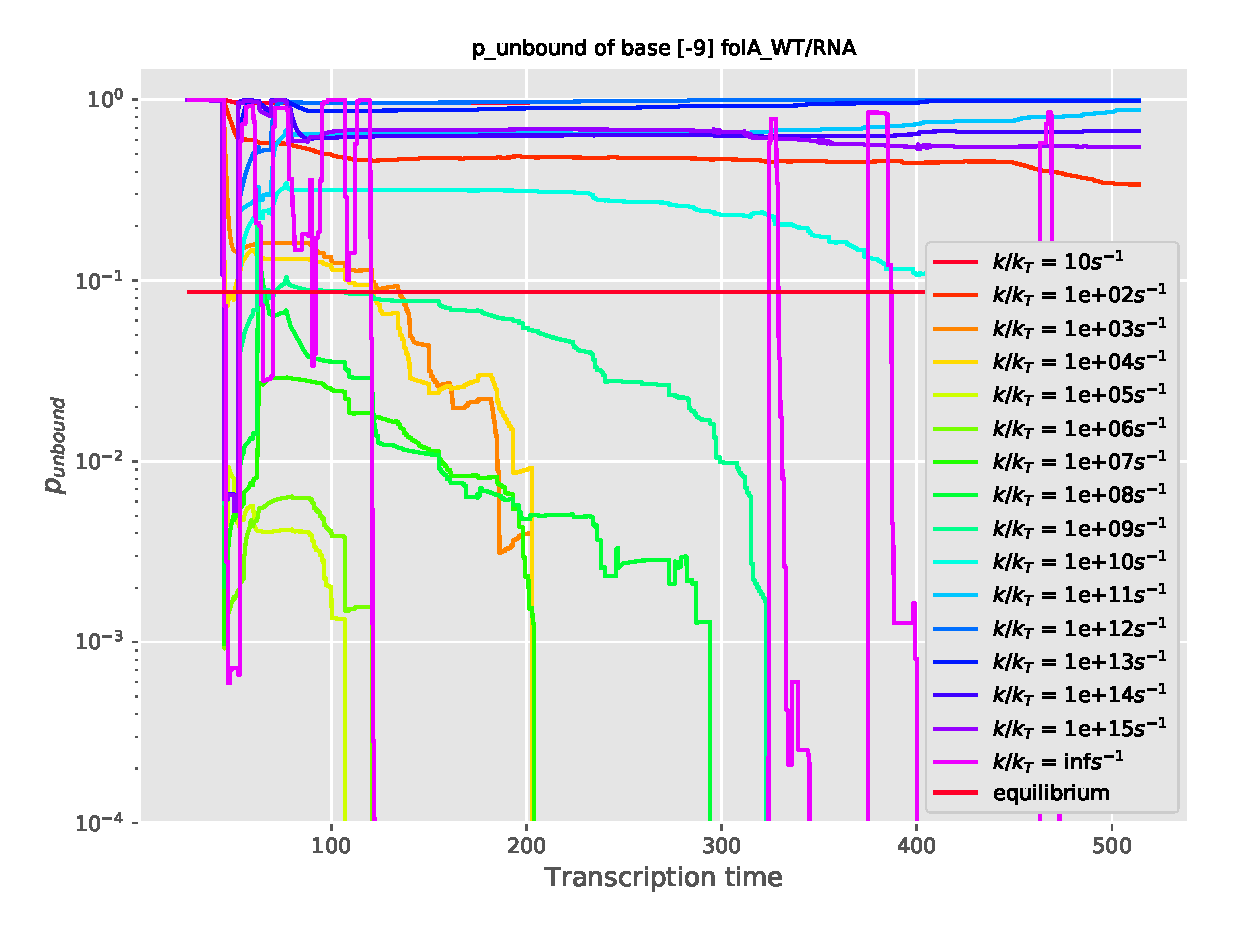
\includegraphics[width=\linewidth]{p_unbound/RNA_p_unbound_base[-9]_k_tuning}
\caption{}
\label{fig:RNA_p_unbound_base[-9]_k_tuning}
\end{figure}
\begin{figure}
\centering
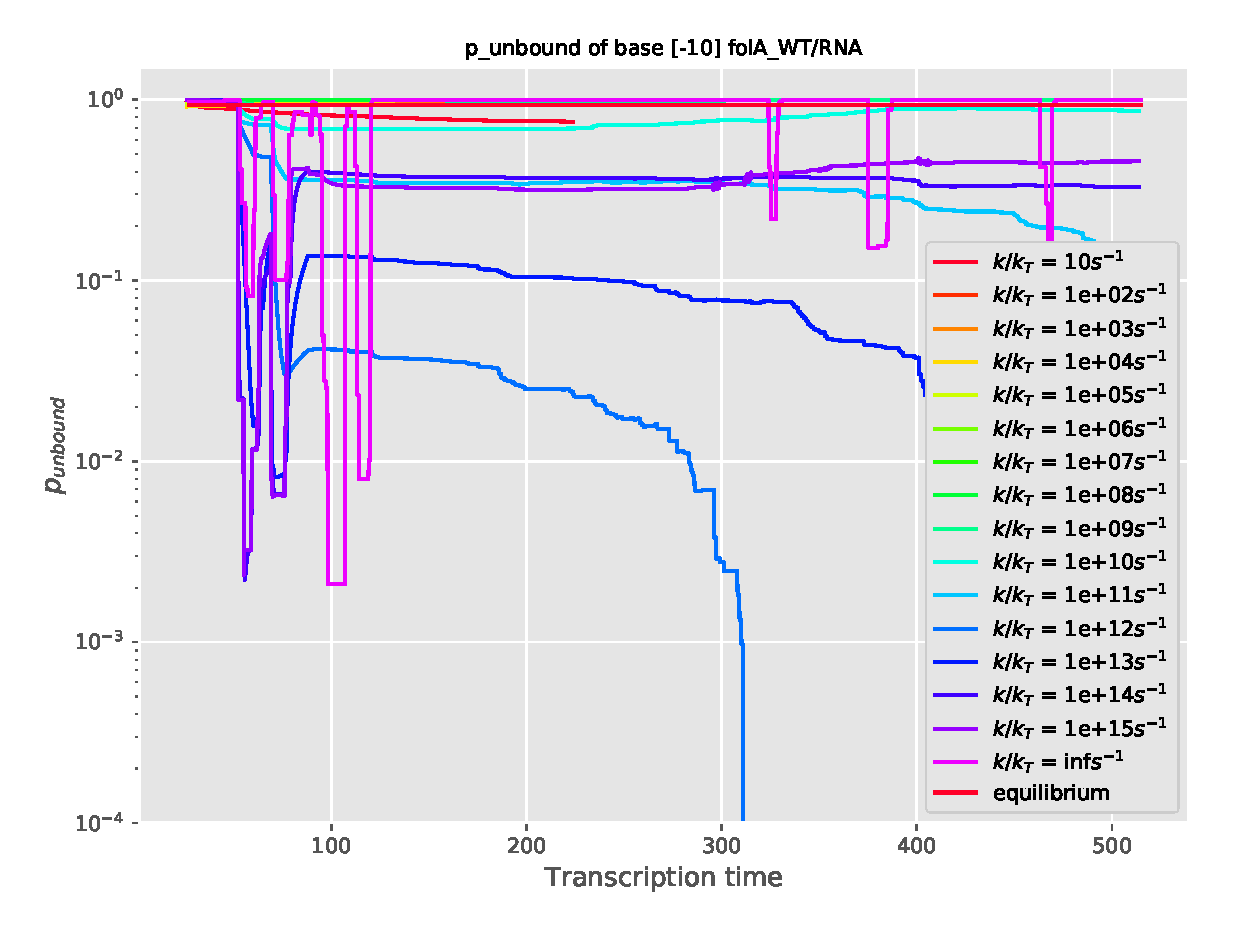
\includegraphics[width=\linewidth]{p_unbound/RNA_p_unbound_base[-10]_k_tuning}
\caption{}
\label{fig:RNA_p_unbound_base[-10]_k_tuning}
\end{figure}
\begin{figure}
\centering
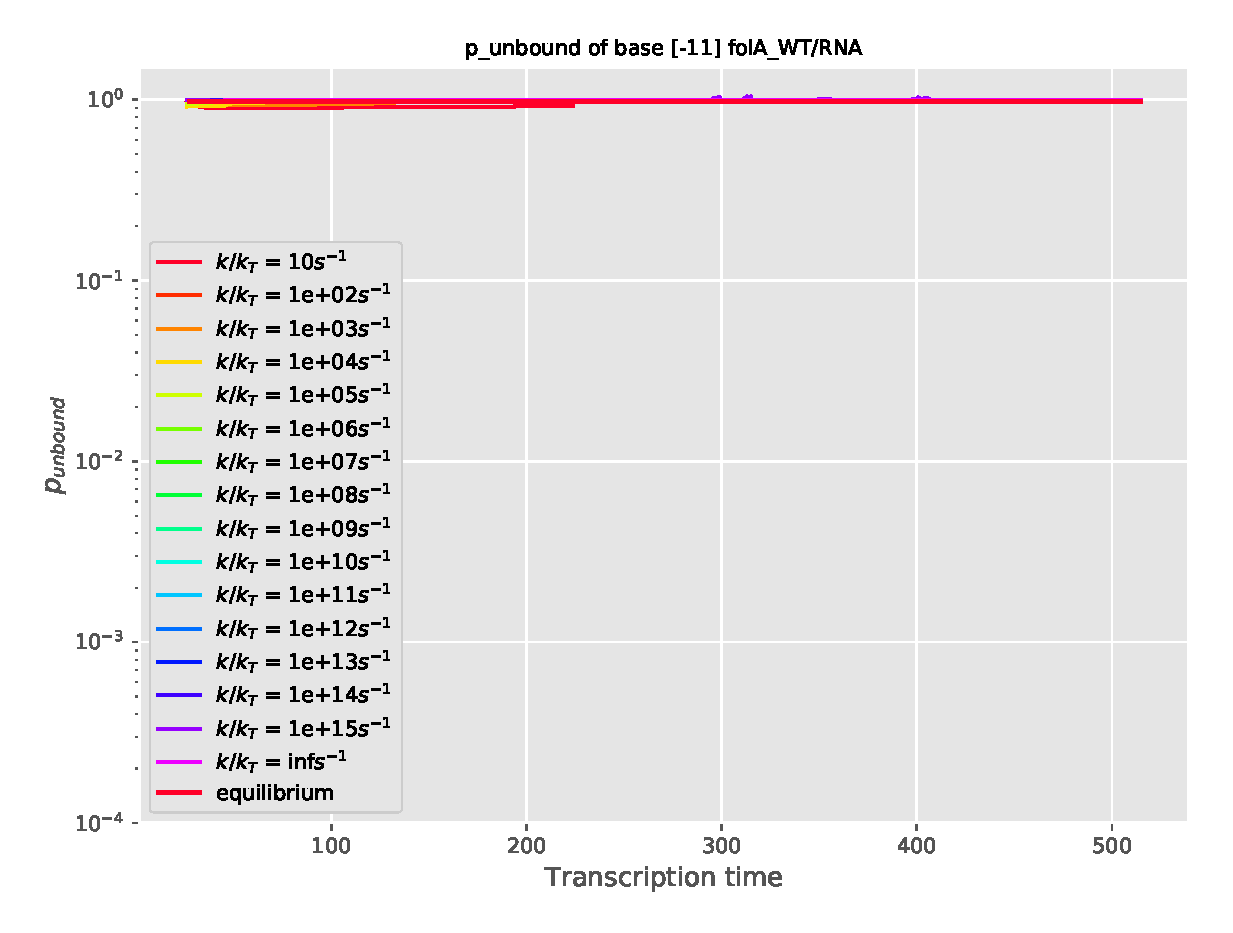
\includegraphics[width=\linewidth]{p_unbound/RNA_p_unbound_base[-11]_k_tuning}
\caption{}
\label{fig:RNA_p_unbound_base[-11]_k_tuning}
\end{figure}
\begin{figure}
\centering
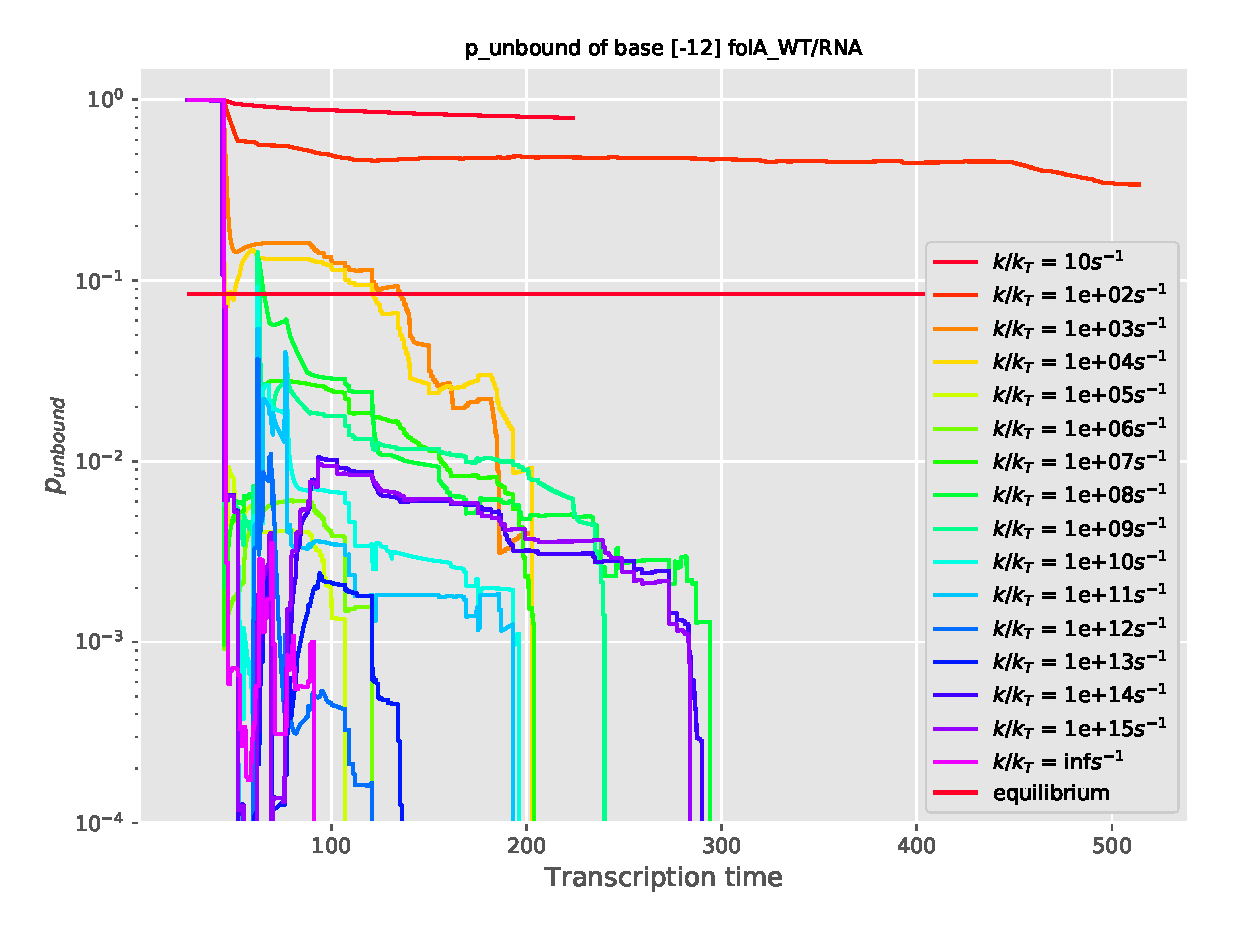
\includegraphics[width=\linewidth]{p_unbound/RNA_p_unbound_base[-12]_k_tuning}
\caption{}
\label{fig:RNA_p_unbound_base[-12]_k_tuning}
\end{figure}
\begin{figure}
\centering
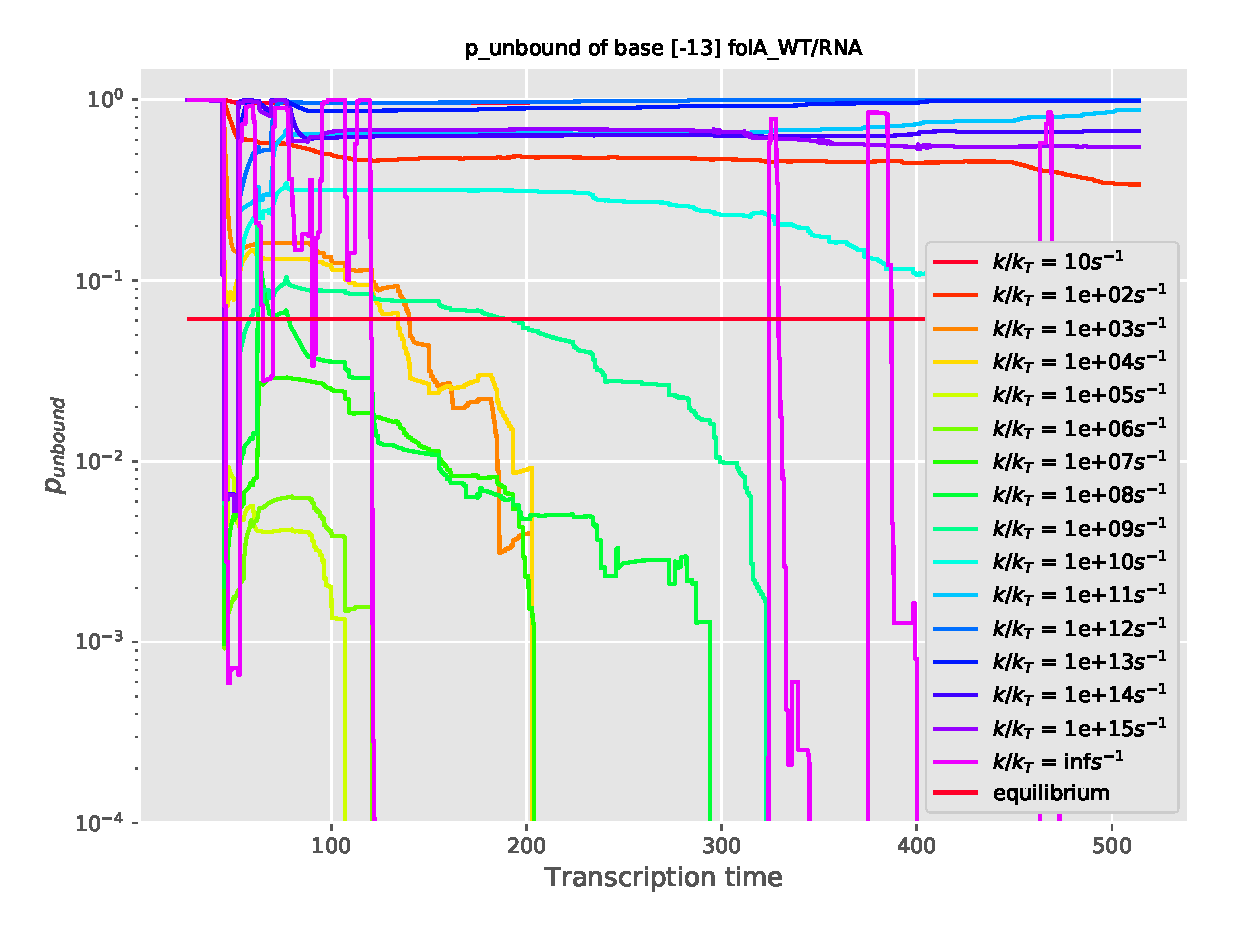
\includegraphics[width=\linewidth]{p_unbound/RNA_p_unbound_base[-13]_k_tuning}
\caption{}
\label{fig:RNA_p_unbound_base[-13]_k_tuning}
\end{figure}
\begin{figure}
\centering
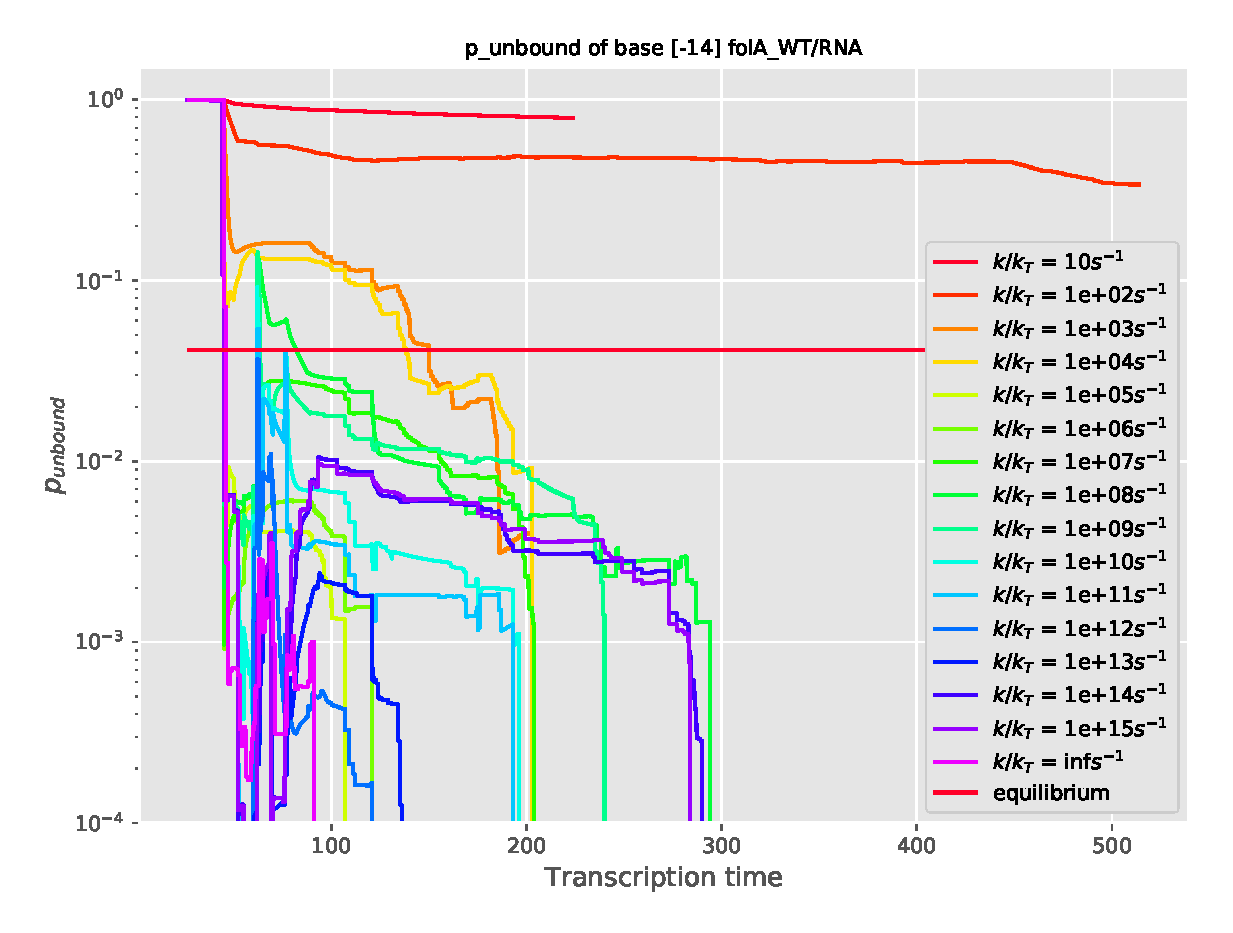
\includegraphics[width=\linewidth]{p_unbound/RNA_p_unbound_base[-14]_k_tuning}
\caption{}
\label{fig:RNA_p_unbound_base[-14]_k_tuning}
\end{figure}


%\paragraph{a.} Using a genetic-algorithm based method and NUPACK to predict populated RNA configurations during cotranscriptional folding (in progress);
%\paragraph{b.} Using master equation method to simulate evolution of folding configurations and SD sequence accessibility.

%In order to examine when the one-dimensional coordinate projection could be recognized as effective reaction coordinate,
%we then examine the probability distribution of committors for transition path trajectories $p(q|TP)$, for which a single peak of probability $p(q|TP)$ have been ultilized as a indicator for 'good' reaction coordinates.
% Firstly, We found that for harmonic toy model, the shape of $p(q|TP)$ is very sensitive to the definition of source/sink region. For illustration, $p(q|TP)$ for two different selection
%  of source/sink regions was compared: in the first case, only two free energy minimum was indentified as source or sink\textbf{(S1)}; in the second case, only the barrier top was
%  defined as the transition path, while other two region of the free energy landscape was calssified as source/sink\textbf{(S2)}.

%\cite{Jacobs2018,Chaudhury2010,Vanden-Eijnden2010,Metzner,Krivov}

\small
%\bibliographystyle{plain}
%\bibliography{0727}

\end{document}
